\chapter{引言}
\section{研究背景和意义}
地震勘探的主要目标是通过观测的地震数据来推断地下结构以及定量地估计介质参数。
弹性参数,包括纵波(P波)速度、横波(S波)速度以及密度等参数,可以通过岩石物理这一桥梁转换为岩石物性参数,从而获得储层及其围岩的岩石性质。这对油气田的勘探、
开发以及二氧化碳(CO$_2$)填埋动态监测等具有重要意义。传统地震数据处理中,通常用声波方程来描述地震波在地下介质中的传播。而地下介质的真实情况往往要复杂得多,
需要通过考虑弹性
、各向异性甚至衰减的波动方程来更准确地描述波的传播。但是介质模型越复杂,所引入的计算量就越大,
所对应的多参数反问题也越困难。目前来看,从声介质过渡到弹性介质能够以较小的代价来获取较准确的模型表征。
尽管从声波近似过渡到弹性近似会成倍地增加计算量,但是这对多分量地震数据的成像或反演显然十分必要。考虑弹性效应的数据处理流程能区分并利用数据中的
P波与S波模式,因此可以充分利用弹性全波场信息改善气云区成像、岩性估计、流体识别以及裂缝与应力场的刻画等。
近年来,岩性油气藏(如致密砂岩、页岩)勘探技术极大地依赖于弹性参数估计,这使得考虑地震波的弹性乃至各向异性效应都具有重要意义。

地震勘探中的诸多过程都非常依赖于速度模型的精度,例如叠前深度偏移、振幅随偏移距变化(AVO)分析等都需要准确的背景速度模型。
因此,如何准确地获取高分辨率的速度模型是地震勘探中最为迫切的任务。
为了降低地震数据与模型参数之间的非线性程度,Claerbout (1985)\cite{Claerbout1985Imaging}将速度模型分解为两个部分:1)描述速度(阻抗)界面的高频部分;
2)控制波传播走时的中低频部分。这样的分解对应于地震勘探中最核心的两个任务,即偏移成像与速度建模。传统方法中,偏移成像和AVO
反演通常用来获取模型的高频部分,
而偏移速度分析(MVA)和走时层析被用来恢复模型的低频部分。但是地面地震反射数据的有限观测孔径以及子波的带限效应使得
这类方法所能恢复的波数谱上存在明显的缺口。如图\ref{fig:GapInSeisVel},
MVA与走时层析只能恢复波数非常低的成分,而偏移成像只能获得有限带宽的高波数信息。
为此,人们也在研究各种方法来尽可能填补速度反演中的波数谱缺口。基于射线理论,有学者尝试采用高分辨率走时层析来拓宽低波数部分的反演能力,
采用真振幅和最小平方偏移方法拓展对高波数成分的反演能力。
但是以上基于射线理论的方法,在模型复杂区域很难处理多路径及焦散等问题。
近年来,随着高性能计算能力的不断提升,基于波动理论的速度反演方法由于可以避免上述问题并具有更高的分辨能力而受到越来越多的关注。
目前基于波动理论的反演方法主要有以下三类:
%许多学者尝试采用高分辨率走时层析、波动方程速度分析(WEMVA)等方法扩展低波数部分的频带,而高波数部分则采用真振幅和最小平方偏移方法来获取更高精度和更宽波数范围的结果。
%同时,更具潜力的全波形反演方法(FWI)采用全波场信息能够获得具有更连续波数谱的地下模型。
\begin{figure}[t] 
   \centering 
   \subfloat{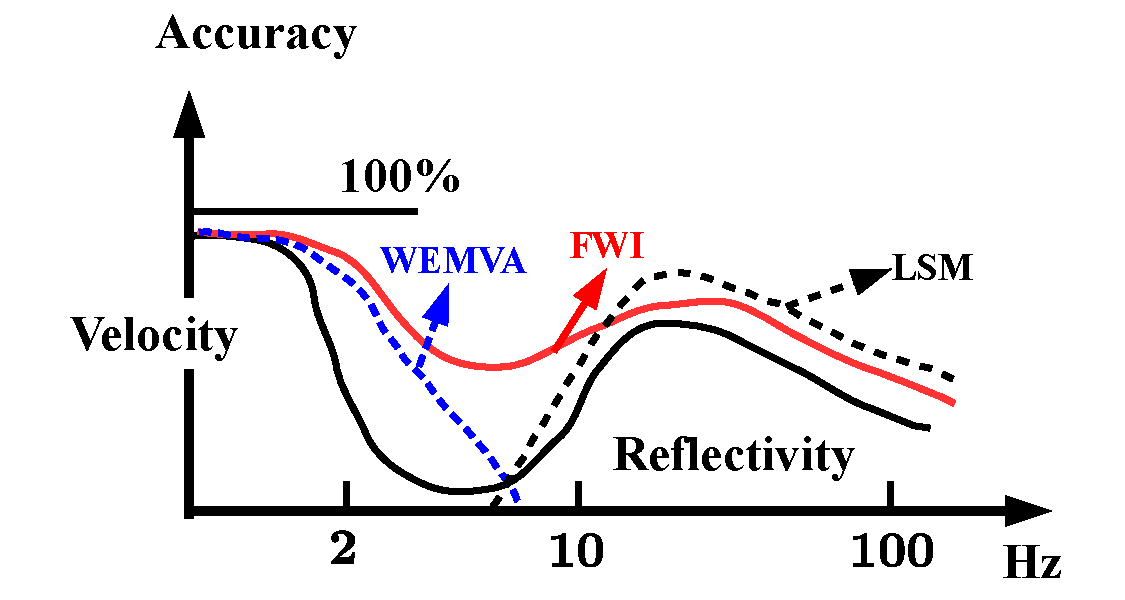
\includegraphics[width=1.00\textwidth]{Figure/chapter01/WavenumberGap2.pdf}}
   \caption{地震数据所能恢复的频带示意图。传统走时层析+偏移成像的方式所恢复的速度模型有明显的中低频缺口,
	   WEMVA和LSM方法有助于拓展低波数与高波数部分的带宽,而FWI则尝试恢复更连续的波数谱(引自Claerbout, 1985\cite{Claerbout1985Imaging})。}
   \label{fig:GapInSeisVel}
\end{figure}

%传统方法中大多基于射线理论进行成像与速度估计,这在模型复杂区域很难处理多路径以及焦散等问题,基于波动理论则可以避免上述问题。
%目前基于波动理论的反演方法主要有以下三类:

1、全波形反演(FWI):该方法通过匹配数据中携带的所有信息,包括走时、振幅、模式转换甚至多次波等,来获得对地下模型全波数谱的
恢复。
相比走时层析和MVA,它可以获取更高分辨率的地下模型。
自从Lailly (1983)\cite{lailly1983seismic}和Taratola
(1984)\cite{tarantola1984}建立了FWI理论框架之后,随着长偏移距、宽方位数据采集的推广,FWI
被认为是填补速度模型中尺度波数缺口最有潜力的工具。
但是FWI也受到众多因素的制约,如初始模型不够好或者数据缺少低频分量时产生的周波跳跃问题(cycle-skipping)、
地面观测数据导致的有限观测孔径问题、地下实际介质的粘弹性和各向异性问题以及高昂的计算代价等等。因此近二十年来,人们一方面尝试采用宽频震源、
鬼波压制等手段获得更加宽频的地震数据,另一方面尝试从目标函数选取、多尺度反演策略等方面降低上述问题的困扰。即便如此,FWI技术的推广应用扔存在许多挑战。

2、波动方程偏移速度分析(WEMVA):该类方法旨在更新背景速度模型,即模型的中低波数成分。
目前主流的做法通常利用地震数据中的反射波信息,通过构建反射波波路径并沿该路径来合理地更新模型中深部。
根据目标函数的残差类型,WEMVA可以分为数据域反演(如Xu et al., 2012\cite{xu:2012};Wu and Alkhalifah,
2015\cite[]{Wu2015b}; Zhou et al,
2015\cite[]{zhou:2015}; Chi et al, 2015\cite{chi2015})和
扩展成像域反演(如Sava and Fomel, 2006\cite{Sava2006}; Almomin and Biondi, 2012\cite{Almomin2012})。
前者采用观测数据与模拟数据间的走时、振幅等信息作为目标函数,后者则通过最大化扩展域成像道集零偏移距的能量来定义收敛准则。
它们与基于射线理论的成像域层析与数据域(非线性)层析方法有许多类似之处,但避免了传统层析流程中繁琐的人工拾取工作。不过,它们
还是会在一定程度上受到cycle-skipping等问题的困扰。

3、最小平方逆时偏移(LSRTM):该方法可以看作是线性化的FWI。在初始模型足够好的时候通过匹配模拟数据与观测数据的振幅来获得地下反
射系数模型。常规偏移成像
采用伴随算子来近似正传算子的逆,从而近似地获得反射率的成像结果。
但是伴随算子通常近似程度太大,所以有学者提出利用最小平方偏移(LSM)迭代获取越来越合理的正传算子的伪逆((Nemeth
et al., 1999\cite{Nemeth1999}; Kühl and Sacchi, 2003\cite{KuehlEtAl2003};
Dai et al.,
2012\cite{DaiEtAl2012})。
其本质上是通过最小化数据残差施加目标函数对模型二阶导数(Hessian)的信息
来获得二阶的收敛效果,从而获得更好的参数扰动反演结果。

重建地下介质的弹性参数模型对地球内部探测与油气藏的勘探至关重要。
相比声波FWI,
弹性波全波形反演(EFWI)能够自动考虑多分量数据中的各种弹性效应并反演得到地下介质的弹性参数,如P波速度($V_p$)和S波速度($V_s$)和密度($\rho$)。
然而在地震反演中考虑弹性效应会大大增加反问题的非线性程度,而且多参数反演
也会受到参数耦合(trade-off)效应的影响,因此
从声波近似过渡到弹性近似使得计算量和反演的困难程度成倍增加。
近年来,
由于计算机能力提升、多分量观测数据的增多,为了解决声波FWI无法回避的问题,考虑弹性甚至各向异
性的全波形反演逐渐成为研究热点。

多分量地震数据中同时含有P波和S波,这两种不同波模式对地下介质有着不同的刻画能力。
FWI中广泛采用的多尺度策略(分频率、分偏移距、分时窗和分散射角)本质上是选取不同的数据子集来逐步加入到反演中。
董良国等(2015)\cite{董良国2015}
指出在FWI过程中,不同的反演阶段采用不同的数据子集可以降低反演的非线性程度。而在弹性波反演中,更加需要根据不同参数
采用不同的数据子集或者不同的反演阶段
采用不同的数据子集,来降低多参数反演的非线性程度,同时也压制参数间的trade-off效应。
近年来不断发展的弹性波波模式分离技术能够提供准确的P或S波数据子集(Zhang and McMechan,
2010\cite{zhang.mcmechan:2010}; Cheng and Fomel,
2014\cite{cheng:2014b}; Li et al., 2016\cite{Li2016a}; Cheng et al.,
2016\cite{cheng:2016}),并已在弹性波逆时偏移(ERTM)中发挥重要作用(Wang et al.,
2016\cite{wang2016scalar})。
这些研究为弹性波反演中采取更多的多尺度策略带来新的机会(Wang et al., 2015\cite{wang:2015}; Ren and
Liu, 2016\cite{ren.liu:2016})。
在弹性框架下,EFWI目的在于构建高分辨率的弹性参数模型,EWERTI则利用弹性波走时信息构建背景速度模型,而ELSRTM是在可靠的背景模型基础上得到
高分辨率的地下反射界面图像。
本文借助模式解耦形成的波场分量或数据子集,实现新的更灵活的多尺度EFWI、EWERTI和ELSRTM方法,以期更准确地估计弹性参数模型的高、中、低波数成分,
为地球内部成像与油气资源勘探提供更好的支撑。

%通过模式解耦获取P或S波数据并根据
%需要加入到不同的反演阶段中,
%这种策略将贯穿始终,
%模式解耦将在EFWI,弹性波波动放程反射走时反演(EWERTI)以及ELSRTM中提供的分离的P或S波数据,来帮助获得更好的反演结果。
\section{研究现状}
\subsection{弹性波全波形反演研究现状}
Claerbout
(1971\cite{Claerbout1971})采用爆炸反射面的概念解释了地震偏移如何对地下构造进行刻画。Lailly
(1983)\cite{lailly1983seismic}
和Tarantola (1984)\cite{tarantola1984}最早用观测数据与模拟数据间波形残差的$L_2$范数作为目标函数,将偏移成像转化为
最优化问题,即FWI问题。该反问题的梯度(方向)可以采用伴随状态法通过入射波场与伴随波场之间的互相关来快速获得。FWI试图将宏观速度模型的
建立与偏移成像两个任务统一在一个流程中,以期在地下每个网格点获得具有连续波数谱的高分辨率图像。但是,早期只利用反射数据的FWI很少有令人满意的
结果。由于短偏移距观测的地震数据对中尺度波长的速度信息非常不敏感(Virieux and Operto,
2009\cite{virieux2009overview}),只有在初始模型非常准确
的时候FWI才会收敛。
从上世纪80年代末期开始,随着FWI技术在长偏移距以及井间透射地震资料的应用中取得成功,
人们才认识到FWI的潜力(Mora, 1987\cite{mora:1987}; Mora, 1988\cite{mora1988elastic}; Pratt
and Worthington, 1990\cite{PRATTEtAl1990}, Pratt et al., 1996\cite{pratt1996two})。
近年来,随着长偏移距、宽方位和宽频带地震数据逐渐增多,基于声波近似的FWI在越来越多的实际数据中获得成功应用,例如Ravaut
et al., 2004\cite{RavautEtAl2004},Operto et al., 2006\cite{Operto2006},Shin et al.,
2009\cite{ShinEtAl2009}。然而即使对于含有长偏移距的数据而言,由于波传播路径的增加,非线性程度变得更加剧烈,因而从FWI中获得稳健的反演结
果仍然受到很大挑战(Sirgue, 2006\cite{sirgue2006importance},Virieux and Operto,
2009\cite{virieux2009overview})。

从前文背景分析可知,最早始于Tarantola (1986)\cite{tarantola:1986}和Mora (1987)\cite{mora:1987}
的弹性波全波形反演能够获得更多地下介质的弹性参数($V_p$, $V_s$和$\rho$)。
尽管需要很大计算代价,EFWI已在很多实际数据中获得了应用(
Crase et al., 1992\cite{crase1992nonlinear}; Djikpesse and Tarantola,
1999\cite{djikpesse.tarantola:1999}; Sears et al., 2008\cite{sears2008}; Sear et al.,
2010\cite{sears:2010}; Prieux et al., 2013a\cite{prieux:2013a}, 2013b\cite{prieux:2013b}; Vigh et al.,
2014\cite{vigh:2014})。
EFWI的实现方式可以在时间域(Shipp et al., 2002\cite{shipp:2002}),
也可以在频率域(Brossier et al.,
2009\cite{brossier2009}),也可以采用混合的方式在时间域进行正演模拟而在频率域求解反问题
(Nihei and Li, 2007\cite{nihei.li:2007}; Sirgue et al.,
2008\cite{sirgue:2008})。然而,EFWI也会受到声波FWI中类似的非线性问题困扰,在海洋环境中(尤其是软海底情况下)由于PS
转换模式非常弱,基于拖缆或者海底多分量数据的EFWI的非线性程度会变得更严重\cite{sears2008}。
同时,不同参数
在特定散射角范围内会产生相似的数据扰动,从而导致不同物理参数之间trade-off效应
(Forgues and Lambare, 1997\cite{forgues.lambare:1997})。
%在海洋环境中,尤其是在软海底环境中,由于PS
%转换模式非常弱,基于拖缆或者海底多分量数据的EFWI的非线性程度会变得更严重\cite{sears2008}。

从声介质到弹性介质,波形反演方法将受到更多挑战。解决EFWI中的这些难题,
不仅要应对原有声波FWI框架下的困难,同时也要解决多参数反演带来新问题。下面分别讨论EFWI面临的两个主要挑战:

1、反演的非线性,也即周波跳跃(Cycle-skipping)问题。FWI是基于Born近似理论导出的。Miller et
al. (1987)\cite{MillerEtAl1987}基于ray+Born理论,
将模型中散射点局部的波数矢量表达为:
\begin{equation}
    \mathbf{k}=\mathbf{k_s}+\mathbf{k_r}=\frac{\omega}{v}cos\frac{\theta}{2}\mathbf{n},
    \label{eq:Modelwnb}
\end{equation}
其中$\mathbf{k}$为照明矢量,$\mathbf{k_s}$和$\mathbf{k_r}$分别是震源端和检波点端的波数矢量,$v$为局部速度,$\theta$为散射角,
$\omega$为角频率,$\mathbf{n}$为$\mathbf{k}$方向的单位向量。由上式可以看出,低频和大张角($\theta$)数据对于中低波数成分的恢复至关重要。
\begin{figure}[!htb] 
   \centering 
   \subfloat{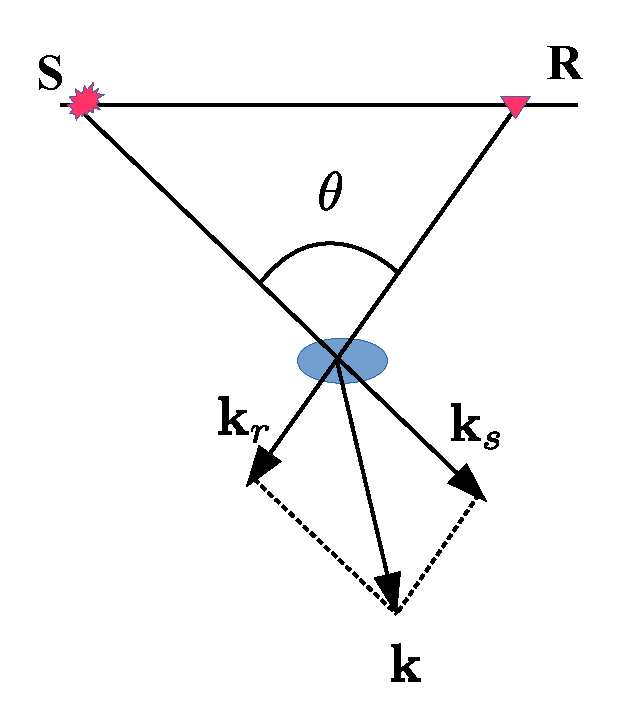
\includegraphics[width=0.40\textwidth]{Figure/chapter01/Wavenumbervector.pdf}}
   \caption{地下散射点处入射波矢量,散射波矢量以及散射角之间关系示意图。}
   \label{fig:WavenumberVector}
\end{figure}
\begin{figure}[b] 
   \centering 
   \subfloat{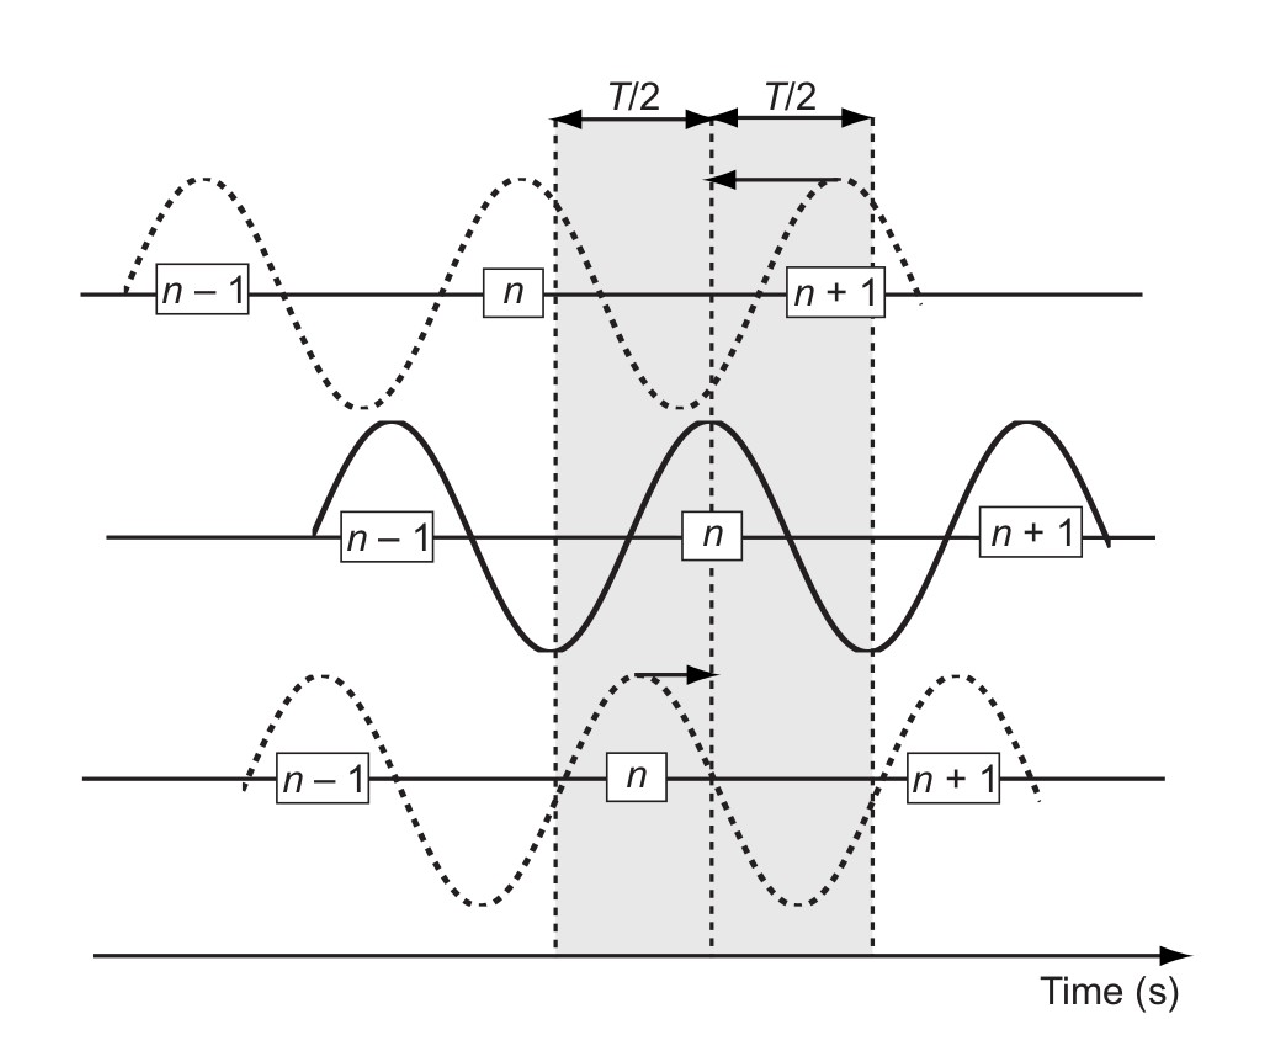
\includegraphics[width=0.60\textwidth]{Figure/chapter01/Cycle-skipping.pdf}}
   \caption{FWI波形匹配中的cycle-skipping现象(Virieux and Operto,
	   2009\cite{virieux2009overview})。当波形相差$T/2$周期以上的时候,数据将会在另一个周期中进行匹配,此时获得的数据残差会导致反演
   陷入局部极值。}
   \label{fig:Cycleskipping}
\end{figure}
因此,FWI的成功与否非常依赖于长偏移距记录和数据中有效的低频分量。如图\ref{fig:Cycleskipping}
所示,如果初始模型不够好导致波形匹配时相差$\frac{1}{2}$周期以上,那么就会使得反演陷入局部极值,这也就是所谓的“周波跳跃”问题。
在声波FWI中,人们发展了许多策略来应对非线性问题,如从低频到高频的多尺度策略(Sirgue and
Pratt, 2004\cite{sirgue.pratt:2004}; 刘国峰等, 2012\cite{刘国峰2012};
刘璐等,2013\cite{刘璐2013}; 曹书红和陈景波, 2014\cite{曹书红2014}; 
张文生等, 2015\cite{张文生2015}),根据时窗与偏移距分选数据子集逐步加入反演中(Shipp and
Singh, 2002\cite{shipp:2002}; Wang and Rao, 2009\cite{WangEtAl2009}; Sears et al., 2008\cite{sears2008}),
修正目标函数使其凸性更好(Luo and Schuster, 1991\cite{luo1991}; Tromp et al.,
2005\cite{tromp2005seismic}; Chi
et al., 2014\cite{ChiEtAl2014}; Wu et al., 2014\cite{Wu2014b}; Shin and Cha,
2008\cite{shin.cha:2008}; Luo et al., 2016\cite{Luo2016})等等。上述策略可以用
在EFWI中,但是由于更多参数的引入以及更复杂的弹性波波场,这些策略需要根据情况择优或者组合使用。

EFWI中不但会出现同样的强烈非线性,而且将面临更复杂的情况。
在构建初始模型的时候要同时获得足够好的$V_p$与$V_s$模型,才能对各种模式的转换波形进行
匹配。
与建立$V_p$模型不同,目前尚未有成熟流程来获得合理的S波速度模型。
许多EFWI方法在研究中都假设$V_s$与$V_p$之间有着固定的泊松比,因此可以通过简单的比例系数
来构建初始模型。但是当地下介质泊松比变化较大时很难获得较好的初始$V_s$模型。
此外,由于相同偏移距下,转换PS波的有效散射角范围相对PP波更小,并且S波速度相对较低等因素会导致EFWI对$V_s$高波数成分的过度更新,
这就又增加了EFWI的困难。
为了降低EFWI的非线性程度,许多学者通过
包络目标函数(Wu et al., 2014\cite{Wu2014b}; 黄超等,2015\cite{黄超2015};
王官超和杜启振,2016\cite{王官超2016}),
或者通过研究目标函数性态来指导多尺度策略的设计
(Brossier et al., 2010\cite{BrossierEtAl2010};王毓玮等,2016\cite{王毓玮2016})。
Tarantola(1986)\cite{tarantola:1986}指出EFWI应分主次顺序依次构建具有不同影响的参数。
也有学者多级地选取不同数据分量来进行多尺度反演(Sears et al., 2008\cite{sears2008}; Operto et al., 2013
\cite{operto2013guided})。然而实践中,诸多因素会制约这些策略的应用,例如低频缺失、初始模型不够好、子波估计困难、噪音干扰等。因此降低EFWI的非线性
程度使反演更加稳健可靠依然需要诸多努力。

2、多参数trade-off效应。如果物理模型中含有多个不同的物理参数,不同的参数扰动可能会引起相似的数据扰动。虽然产生的数据扰动可能不完全一致,
但是不同参数扰动产生的散射波场会在特定角度范围内重叠,这就导致常规的地面观测数据通常无法区分数据扰动来自哪一种
参数扰动,从而引起参数间的trade-off效应。这样的话,即使在初始模型足够好的时候也很难从数据扰动中恰当地恢复相应的参数扰动。

为了解决EFWI中的trade-off问题,
许多学者通过调查散射模式或者Hessian算子来选取不同的参数化方式(Wu and Aki, 1985\cite{wu.aki:1985}; Tarantola, 1986\cite{tarantola:1986}; 
Plessix and Cao, 2011\cite{plessix.cao:2011}; Gholami et al, 2013\cite{gholami2013})。
当然,最有效的就是考虑多参数Hessian算子,用Hessian的信息来压制trade-off的影响(Fichtner et al., 2001\cite{fichtner2011hessian}; Operto et al.,
2013\cite{operto2013guided}; Pan et al., 2015\cite{pan2015estimation}; Yang et al.,
2016\cite{Yang2016})。然而Hessian有关的计算所需代价太过昂贵,即使在声波FWI中也很难在大规模问题中获得应用。在EFWI中想要压制参数trade-off,就
需要在反演中利用Hessian非对角区块的信息。近期,在Hessian非对角区块的近似与利用方面,许多学者做出了一些有益的尝试,例如Wang
et al. (2016)\cite{WangYuweiEtAl2016}采用块对角Hessian压制参数耦合。Pan et
al (2017)\cite{PanEtAl2017}借助l-BFGS优化策略进行多参数反演。
Wang et al. (2015)\cite{wang:2015}和Ren and                                                                           
Liu
(2016)\cite{ren.liu:2016}初步讨论了基于弹性波模式解耦的梯度预条件方法及其在压制参数trade-off效应中的潜力。
Wang and Cheng (2017)\cite{WangEtAl2017}进一步对比了模式解耦与Gauss-Newton预条件梯度的差异,
指出模式解耦可以部分地利用Hessian非对角块来压制P波对$V_s$反演的干扰。由于常规地震观测很难敏感地捕捉密度信息,至今密度
的反演依然非常困难(Jeong et al., 2012\cite{jeong2012full}; Prieux et al., 2013\cite{prieux:2013a}; Yang
et al., 2016\cite{Yang2016})。
\subsection{弹性反射波波形反演研究现状}
常规FWI在长偏移距、宽方位数据中有着不错的效果,但主要是利用了透射波以及临界反射波所携带的信息来更新速度模型的
中低波数分量。由于FWI的成功非常依赖这些波场信息,使得地震数据往往缺乏足够的大偏移距信息来更新中深部结构的中低波数成分。
换句话说,在中深部区域,FWI往往过多地更新来自反射数据的高波数成分(相当于最小平方偏移)。从式\eqref{eq:Modelwnb}
可以看出,在相同频率和速度情况下,深部的反演需要更大的角度孔径才能确保足够的低波数照明,这也意味着要更大的偏移距。然而,即使
采用现有宽方位、长偏移距观测也很难保证这样的覆盖,而且更长的偏移距也意味着更强的非线性\cite{sirgue2006importance,virieux2009overview}。

利用反射波信息可以更好地照明深部结构。通常,可以在成像域或者数据域实现基于深部反射波的速度更新。在成像域,该类方法通常被称为偏移速度分析(MVA),主要利用拉平
共成像点道集作为收敛准则。
在实际生产中,通过反射走时层析来反演反中深部的背景速度已经是非常成熟的技术(Woodward,
1992\cite{Woodward1992}; Meng et al., 2004\cite{MengEtAl2004}; Woodward et al., 2008\cite{
Woodward2008}; Jones, 2010\cite{Jones2010})。
它通过将共成像点道集上的剩余时差(或深度差)反投影到射线或Born波路径上来更新速度。不过基于射线理论的走时层析经常需要进行一些人工拾取,比如在每轮迭代中进行
成像剖面与成像道集剩余曲率的拾取。在构造复杂区域,高频渐近假设失效,使得射线走时层析的有效性明显下降。
基于波动理论的WEMVA可以很好地应对上述问题,但是通常
需要借助昂贵的扩展域成像,通过最小化非零偏移距的能量来实现模型更新,如Sava and
Fomel (2006)\cite{SavaEtAl2006}; Yang and Sava(2011)\cite{YangEtAl2011}; Almomin and
Biondi(2012)\cite{Almomin2012}; Sun and Symes(2012)\cite{SunEtAl2012}。尽管WEMVA在
二维应用中取得了不错的效果,但三维应用中过高的计算成本是一个明显的制约因素。
%一方面偏移成像需要大量计算,
%另一方面扩展成像条件的施加同样耗费极大。
针对反射走时,Luo et
al. (2016)\cite{Luo2016}用时间轴方向的扩展成像与Rytov近似结合,提出了全走时反演(FTI)方法并在理论合成数据上
获得了不错的反演效果。该方法实质上也是一种成像域的速度反演方法。

在数据域同样可以利用反射波对模型深部进行更新。
有些学者(Chavent et al., 1994\cite{ChaventEtAl1994}; Plessix et al., 1998\cite{PlessixEtAl1998}; Clment et al., 2001\cite{ClementEtAl2001})
将速度模型分成高波数(反射率)与低波数(背景模型)成分,提出了偏移成像走时层析(MBTT)方法。
从Alder (2008)\cite{Adler2008}提出的基于射线理论的非线性层析方法出发,Wang
et al. (2014)\cite{WangEtAl2014}和Yang et al.
(2016)\cite{YangEtAl2016}采用一次偏移后拾取+图偏移的方式建立叠前数据的不变量(如走时,出射慢度等),
通过对
叠前数据不变量的多次拟合来更新层析速度模型,既减少了人工拾取,又达到加快收敛的效果。

基于波动理论的数据域速度反演近年来受到了广泛的关注。
受MBTT方法的启发,Xu et al. (2012)\cite{xu:2012}提出了反射波波形反演(RWI)方法。它先采用RTM或LSRTM获取反射率模型,
然后用Born模拟(反偏移)来预测反射率所产生的反射波。反射波与背景波场的互相关可以得到反射波波路径(敏感核函数)信息。
RWI的关键就是将数据残差反投影到反射波波路径上,从而更新模型分量的中低波数成分。
RWI方法出现后,许多学者做了大量研究,采用了波形拟合的$L_2$范数,如Xu
et al. (2012)\cite{xu:2012}, Wang et al. (2013)\cite{Wang2013}, Wu and
Alkhalifah (2015)\cite{Wu2015b},
Zhou et
al. (2015)\cite{zhou:2015}。
近期,Irabor and
Warner (2016)\cite{Irabor2016}和Wang et al.
(2016)\cite{WangFangEtAl2016}通过上、下行波分离来帮助常规FWI获取背景分量的更新,其实质也利用了反射波波路径的信息。
%然而,尽管RWI的目的在于更新背景速度,波形拟合的$L_2$范数在背景速度与真实值相差较远的时候,反偏移
%所预测的与
然而,尽管RWI的目的在于更新背景速度,当背景速度与真实值相差较远的时候,反偏移
所预测的与观测数据中的反射波波形也可能相差半个周期以上,从而导致波形拟合的$L_2$范数产生周波跳跃。Wang et
al
(2013)\cite{Wang2013}指出采用低频数据可以一定程度上缓解跳周现象。为了避免振幅相关的目标函数带来的非线性,更趋于线性关系的
走时类目标函数获得了关注。Ma and
Hale
(2013)\cite{ma2013}采用动态图像识别(DIW)来获得模拟与观测反射数据之间的时移量,从而提出了波动方程反射走时反演(WERTI)方法。类似的,Chi
et al. (2015)\cite{chi2015}和Wang et al.
(2015)\cite{Wang2015}采用互相关类的方法来获取模拟与观测反射数据同相轴的时移(或空移)量。
以上有关RWI的研究都是基于声波方程的。

在弹性反射波反演研究中,目前只有Guo and
Alkhalifah (2016)\cite{Guo2016}将Wu and
Alkhalifah (2015)\cite{Wu2015b}的声波RWI思路进行了扩展。
对于弹性反射波形反演(ERWI),除了声波RWI中面临的问题,还需要处理更多的复杂情况,如多参数trade-off、模式转换、更复杂的反射记录以及
$V_s$反演的困难等。为了应对这些问题,
%利用波模式解耦来分别获取P与S反射波然后应用到RWI或反射走时反演(RTI)中将是非常直观的思路,
本文第四章将论述怎样借助弹性波模式解耦与多分量记录P/S分离来建立比较有效的ERWI方法与流程。
%考虑到弹性波的哪些特殊情况,以便获得可行的ERWI方案。
%许多研究通过选取不同的目标函数来选取方法对应不同名称的反演方法,但核心思想都是一致的

\subsection{弹性波最小平方逆时偏移研究现状}

目前有许多成像方法,如Kirchhoff偏移、高斯束偏移和逆时偏移(RTM)等可以用来恢复地下界面结构形态。
但是随着需求的变化与技术的进步,构造信息已经不能满足勘探的需要。人们想要
获得更高分辨率的弹性参数以便直接或间接用于岩性/流体区分等更高级的任务。
常规FWI算法可以用于参数模型的高分辨率成像(反演),但是会受到许多因素困扰,
如初始模型不好或者数据低频缺失导致的cycle-skipping问题、地震子波未知、正演算子不准确等等。
而且,常规FWI一般需要从低频到高频逐步恢复连续的波数谱。如果单纯想获得模型高波数成分,
用FWI方法就太过复杂或困难。除FWI之外,通常也会通过最小平方偏移(LSM)来实现高波数成分的重构。
早期,Beylkin
et al. (1985)\cite{BeylkinEtAl1985}和
Bleistein (1987)\cite{Bleistein1987}等学者通过广义Radon变换来导出Kirchhoff成像中的振幅校正因子,实现所谓的真振幅成像。
该方法通过射线理论计算Green函数,正问题采用Born近似
,可快速地迭代求解反问题。
针对Kirchhoff偏移,Schuster(1993)\cite{Schuster1993}提出了应用于井间数据的LSM算法,而后Nemeth et al.
(1999)\cite{Nemeth1999}将该方法应用到了地面数据中。

以波动方程为引擎的最小平方逆时偏移(LSRTM)近年来一直是研究的热点,
尽管其计算代价昂贵,但可以处理复杂非均匀介质中所产生的多路径问题。
LSRTM通常可认为是线性的全波形反演。线性近似下若能获得Hessian矩阵的逆算子就可以通过施加逆算子快速获得反问题的解。
但是Hessian的计算与求逆在实际问题中非常困难,
故在空间域采用Hessian的近似来校正成像结果是一种快速实现LSRTM的方法(Chavent and Plessix, 
1999\cite{ChaventEtAl1999}; Shin et al., 2001\cite{shin2001improved}; Symes,
2008\cite{Symes2008})。然而,这种方法在复杂介质中并
不总是有效。另外一种方式是通过在数据域求解目标函数的最小化问题。
假设在已经获得足够好的低波数模型成分之后恢复模型的高频扰动,即获得“像”或
反射率,使得在最小平方意义下,用该反射率所预测的反射数据能与观测数据达到最佳匹配。
这一过程与在单次迭代中通过计算二阶伴随状态方程实现基于
Gauss-Newton法(Bae et al., 2012\cite{bae2012frequency}; Metiver et al.,
2014\cite{Metivier2014})的FWI是一致的。
因此,最小平方逆时偏移与全波形反演的理论框架基本是一致的,只是输入数据(反射波/全波场)和输出结果(高频扰动/模型参数)不一样。
因此目前LSRTM研究中主要通过最小化Born模拟的反射数据与观测数据之间的残差来改善成像质量,获得更高分辨率的反射率、波阻抗
界面或弹性参数扰动的反演结果(Dai and
Schuster, 2013\cite{Dai2013}; Dong et al., 2012\cite{Dong2012}; Luo and
Hale, 2014\cite{Luo2014})。

许多学者针对LSRTM中的其他问题也做了大量的研究工作。Wong et al.
(2015)\cite{WongEtAl2015}将自由表面多次波加入到成像条件中,进而增加地下照明。Zhang et al.
(2015)\cite{ZhangEtAl2015}选取零延迟互相关目标函数来减弱子波估计不准以及振幅描述不准带来的非线性。刘玉金和李振春
(2015)\cite{刘玉金2015}基于成像域的速度反演方法(Symes, 2008\cite{Symes2008a})
在扩展域进行LSRTM,在速度不准确的情况下仍然可以得到合理的成像结果。
近期,为了更准确地描述波传播过程,同时获得更多的参数成像,原本基于常密度声波方程的
LSRTM被推广到了变密度声波介质(Yang et al, 2016)\cite{Yang2016}、衰减介质(Dutta and
Schuster, 2014\cite{DuttaEtAl2014}; 李振春等,2014\cite{李振春2014}; Dai et al.,
2015\cite{Dai2015})以及弹性介质中(Duan et al., 2016\cite{Duan2016}; Feng and Schuster,
2016\cite{Feng2016}; Xu et al., 2016\cite{Xu2016}; Ren et al., 2016\cite{RenEtAl2016})。

相比声波成像,弹性波成像可以提供更多的地下信息,例如转换横波成像可改善气云区成像,有助于区分岩性和识别流体。
但是,许多问题会很大程度上影响弹性波成像质量。
首先,传统声波成像方法中观测孔径限制、粗网格采样、低频噪音以及数据缺失引起的偏移假象同样会出现在弹性波成像中;
其次,记录中的P与S波数据很难完全区分开,泄漏的波模式会引起假象,即“cross-talk”;
再次,一般的成像条件会导致转换波图像的极性反转问题,因此需要选取合适的校正方法(Du et al,
2014\cite{DuEtAl2014}; Gong et al, 2016\cite{GongEtAl2016}; Rocha et al,2016\cite{RochaEtAl2016a})。
%常规ELSRTM可以较好的压制由于观测和数据不完备造成的成像噪音,同时对cross-talk也有一定的压制作用。
%为了解决
%波模式完全区分开,因此其中某些波模式的会因速度不对而被错误地成像。这些非物理的模式就会引起假象,也即“cross-talk”。
%而通过ELSRTM则可以提高成像的分辨率,并且可以压制由于观测孔径限制,粗网格采样以及数据缺失引起的偏移假象。
%弹性波成像需要处理矢量波的问题,也就需要选取合适的成像条件(Du et al, 2014\cite{DuEtAl2014};Gong et
%al, 2016\cite{GongEtAl2016};Rocha et al,2016\cite{RochaEtAl2016a}),
近期Wang et al(2016)\cite{WangChenlongEtAl2016}面向各向同性与横向各向同性(TI)介质提出了
更具有物理含义的无极性反转的矢量成像条件。
最近,从EFWI理论框架出发,有学者(如Duan et al., 2016\cite{Duan2016}; Feng et al., 2016\cite{Feng2016} 等)
推导出了与EFWI梯度非常类似的成像条件,可以回避极性反转问题。
基于第二章对EFWI算法的分析,模式解耦带来的好处同样能在ELSRTM中发挥作用,尤其是压制传统弹性波成像中模式串扰引起的假象。


\section{研究内容}
基于多分量地震数据重构弹性参数模型是本文的重点。
除了层析成像与WEMVA方法之外,目前主流的模型参数估计方法包括FWI、RWI和LSRTM。
我们将以上三种方法扩展到弹性介质,采用EFWI构建高分辨率弹性参数模型,采用EWERTI通过弹性波走时信息构建中深部的背景弹性波速度,
而在可靠的初始弹性速度模型基础上采用ELSRTM构建模型的高波数成分(反射界面的高分辨率图像)。
整个论文中,弹性波模式解耦将是其中最核心的方法,为不同分辨率的弹性参数反演提供解耦的P与S波数据子集,
从而降低反问题的非线性程度、压制参数间trade-off效应。
%以利用由此带来的降低参数间trade-off的便利。
本文下面几章将分为以下四个部分来详细展开:

第二章将通过模式解耦对EFWI梯度进行预条件,降低反演过程中的参数trade-off程度,并达到加速收敛的效果。
首先,通过弹性波Born近似,分析$V_p$与$V_s$扰动的
辐射模式,并给出解耦的Frech{$\acute{e}$}t导数(Jacobian矩阵)。然后,调查解耦后的P波与S波数据对梯度的贡献并提出在梯度计算中的交叉项近似。
在此基础上,通过伴随状态法快速计算得到预条件的梯度,
即正传波场与解耦后反传波场的零延迟互相关。
然后,为了获得更多物理机制上的认识,将计算并分析基于解耦的Hessian和分辨率矩阵,同时也对比模式解耦预条件的梯度与Gauss-Newton(GN)梯度的异同。
接着,利用流体饱和砂岩模型以及Marmousi-II模型的数值算例验证基于模式解耦的EFWI的有效性。
最后,将讨论引入密度给反演带来的复杂性以及模式解耦EFWI的表现。

第三章将通过弹性波波动方程反射走时反演(EWERTI)来重建速度模型中深部的中低波数分量。
文中采用反射波走时拟合差作为目标函数进行反演,其中的走时残差将通过DIW方法来获取。
沿用RWI的思路,通过Born模拟来构建反射波关于背景速度的核函数,即反射波波路径。
参照Ma and Hale (2013)\cite{ma2013}的方式,推导出弹性波反射走时反演的伴随震源与梯度。
通过目标函数的性态分析调查EWERTI的稳健性与收敛性。然后基于反射核函数观察不同反射波波模式对反射波路径的影响。
为了克服反演中的非线性以及P波与S波速度之间的trade-off,将分两个阶段来分别恢复$V_p$与$V_s$:首先,采用PP波反射走时来重建$V_p$背景模型;
然后,在获得足够好的背景$V_p$后,再采用分离出的PS波反射走时重构$V_s$背景模型。
在此过程中,本文提出用地面多分量数据P/S分离来帮助获取PP或PS的走时残差,用空间波场模式解耦来预条件目标函数关于$V_p$或$V_s$的梯度。
最后将在Sigsbee2A模型上进行算法验证。

第四章将采用ELSRTM来获取弹性参数模型的高波数分量。首先,从反演框架出发,建立Born模拟与观测反射数据之间的最小二乘拟合目标函数,
利用矩阵形式的弹性波方程通过拉格朗日乘子法获得伴随状态方程,并导出ELSRTM的梯度公式。
之后根据第二章的推导,利用波模式解耦对梯度进行预条件处理。
由于不同模型的参数耦合程度不同,将根据具体情况设计不同的反演策略。简单模型和Marmousi-II模型的数值实验将用来验证
策略的有效性。
此外,由于ELSRTM基于Born近似,Born正演数据与反射数据之间存在差异。文中也对比了采用Born模拟数据与反射数据反演结果的差异。
%LSRTM为线性FWI过程,反问题的复杂程度将大为降低,
%此外,根据不同模型的trade-off程度设计不同的反演策略,并将对比这些策略在解决参数耦合问题的效果。
%简单模型与Marmousi的数值实验将用来验证算法的有效性。

第五章将对本文的工作进行总结,指出论文的创新与不足之处,并给出下一步的研究计划。
